% Workshop draft — §4. Write this before §5.2 / intro.
% Numbers: output/c3_control/metrics.json (ERP2, src=1626, W=512).

\section{Sparse Temporal Sampling Fabricates Camera Motion}
\label{sec:sparse-sampling}

Compensated-frame temporal seam carving needs an estimate of inter-frame
camera motion: the previous seam is warped by that estimate before it
regularizes the current frame. On equirectangular (ERP) video a camera yaw
is a cyclic horizontal shift, so a natural estimator is phase correlation
on the equatorial band. We report that this estimator, applied to
temporally \emph{sparse} ERP frames, returns confident motion that does not
correspond to camera motion. A three-condition control on a single real
frame shows that the failure is induced by the sampling interval, not by
the estimator and not by the projection.

\paragraph{Estimator.}
Phase correlation is computed on the equatorial band of a full ERP frame
(the polar 15\% of rows are excluded from the correlation, by design: that
is where a yaw is a cyclic shift). Photometric scores use the same band.
No Hann window is applied along $x$, so wrap-around remains a valid shift.

\paragraph{Control.}
We fix one real ERP frame $I_t$ (clip ERP2, source index 1626, width 512)
and run that same estimator under three conditions. Throughout, two
numbers describe the sparse-sampling phantom and must not be read as
two different findings: over the clip's linspace pairs the mean absolute
pan was $141$\,px; the control below uses the \emph{worst} pair, whose
estimate is $253$\,px. The mean is illustrative; the worst pair is the
proof that fabrication occurs in an individual pair, not as a smear of
truth with noise.

\begin{enumerate}
  \item[(A)] \textbf{Known cyclic yaw.}
  We synthesize ground-truth yaw by cyclically rolling the \emph{entire}
  spherical image---poles included---by $k$ pixels,
  $k \in \{8,16,32,64,128,141\}$. The estimator still sees only the
  equatorial band, but that band is taken from a full ERP that has
  undergone a real yaw of a real panorama, not from a cropped planar
  patch. If polar distortion made even equatorial phase correlation
  illegal on this projection, (A) would fail. It does not: the estimator
  recovers each $k$ exactly, and the post-warp photometric residual is
  zero. The tool is correct on this projection when the motion is a
  genuine yaw.

  \item[(B)] \textbf{True consecutive frame} ($\Delta t = 0.03$\,s).
  Estimated pan $0.00$\,px; equatorial dense-flow $u$ $0.00$\,px. Raw
  photometric residual is already $0.36$; warping does not change it
  (ratio $1.00$). At video rate there is no motion to fabricate, and
  none is fabricated. Dense flow is used only here, where a
  stride-$1$ matcher is valid.

  \item[(C)] \textbf{Original linspace neighbor}
  ($\Delta t = 7.74$\,s; $232$ frames---the gap that produced our earlier
  temporal tables).
  The estimator returns a confident pan of $253$\,px (worst pair; clip
  mean $141$\,px). Warping $I_t$ by that shift leaves the equator
  essentially unchanged: photometric residual falls only to $0.95$ of
  raw ($56.2 \rightarrow 53.5$).
\end{enumerate}

\begin{figure}[t]
  \centering
  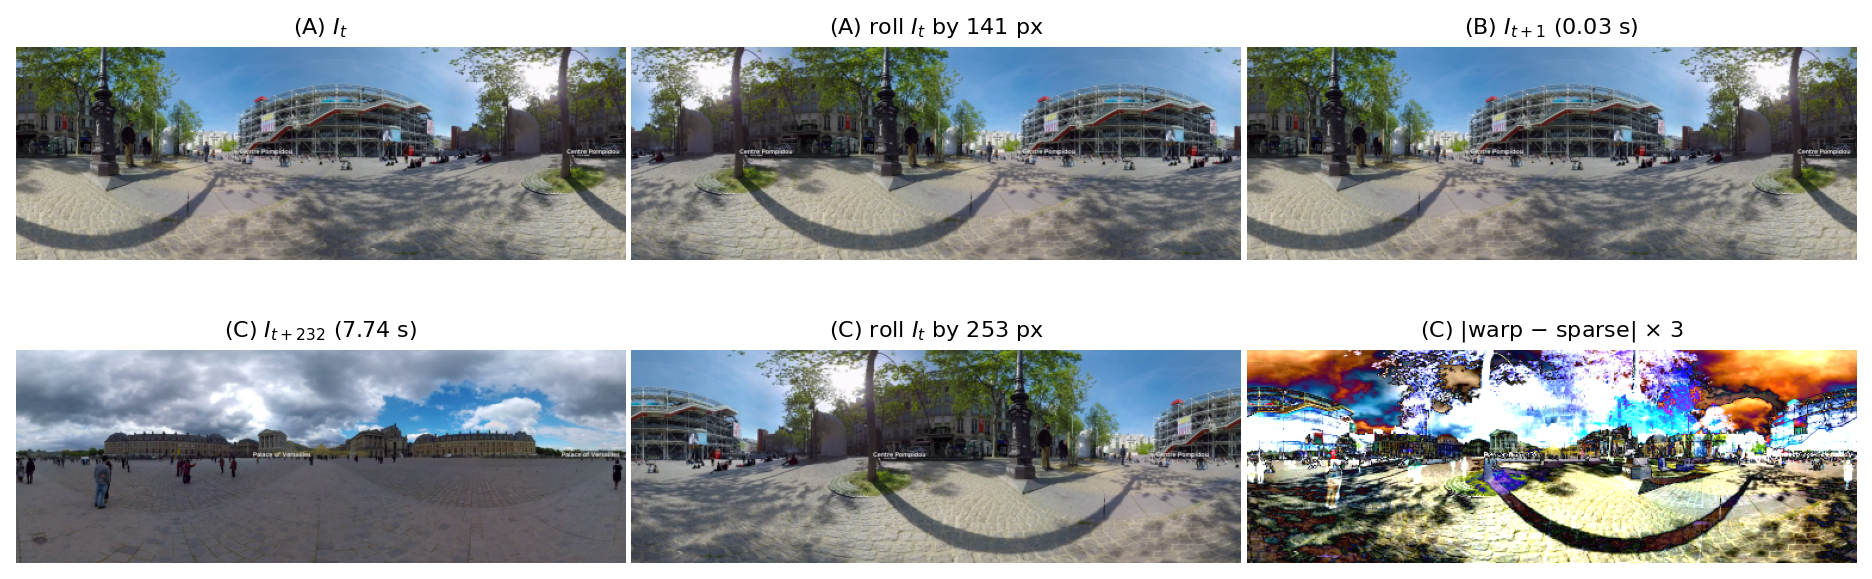
\includegraphics[width=\linewidth]{figures/fig_c3_control.png}
  \caption{Same frame $I_t$ (ERP2, source 1626), equatorial band.
  (A)~A known $141$\,px cyclic roll is a visible shift the estimator
  recovers exactly. (B)~The next video frame is already aligned
  (pan~$0$). (C)~At $7.74$\,s the estimator reports $253$\,px, but
  rolling $I_t$ by that amount does not explain the sparse neighbor
  (residual panel). The fabrication is the gap, not the tool.}
  \label{fig:c3-control}
\end{figure}

\paragraph{Why $0.95$ is not 5\% real yaw.}
A warp that explained camera motion would drive the residual toward zero,
as it does exactly in (A). That it does not means the $253$\,px shift does
not account for the change between the two frames. The few percent of
residual that \emph{does} disappear is expected with no camera motion: over
$7.74$\,s the scene content itself changes (people move; the camera need
not), so any plausible horizontal shift will coincidentally reduce a
little photometric error. Post-warp photometry, not the reported pan
magnitude, is therefore the test of whether an estimate reflects camera
motion. Dense optical flow is not a substitute arbiter at this interval:
DIS and comparable methods are not $7$\,s matchers. We report dense $u$
on (C) only to record that it is undefined as ground truth there
($u \approx 45$\,px); we do not treat it as the true yaw.

\paragraph{What this does and does not show.}
The estimator is correct at both extremes it is designed for---a real yaw
(A) and true adjacent frames (B)---and fabricates a confident,
photometrically unsupported estimate only at the $7.74$\,s sampling
interval (C). This is a statement about the \emph{assumed motion}: it is
absent from this corpus at video rate, and sparse linspace sampling
manufactures a phantom version. It is not a test of whether temporal seam
carving works when genuine inter-frame yaw is present. We did not reject a
temporal method; we found that the problem such a method would regularize
does not occur in these clips, and that a common preprocessing choice
(linspace frames over a long clip) will invent it.

On consecutive-frame windows of ERP2, ERP4, and ERP5 in this corpus, the
same estimator and dense flow agree near zero; we found no
validated-fast yaw window. Residual seam jitter against a pan-warped
predecessor is only as trustworthy as that pan: on linspace pairs it
inherits the fabrication in (C).

Any pipeline that estimates inter-frame motion from temporally sparse
$360^\circ$ samples---a usual consequence of linspace frame selection over
long clips---risks warping seams by motion that was never present.

Validate estimated motion against post-warp photometry before use, and
sample at true video rate when temporal consistency is the objective.
